\documentclass{svproc}
\usepackage{url}
\def\UrlFont{\rmfamily}
\usepackage{graphicx}
\usepackage{float}
\usepackage{amsmath,amssymb,amsfonts}
\usepackage{textcomp}
\usepackage{xcolor}
\usepackage{booktabs}
\usepackage{array}
\usepackage{multirow}
\usepackage{siunitx}
\usepackage{pgfplots}
\usepackage{hyperref}

\pgfplotsset{compat=1.18}
\sisetup{round-mode=places,round-precision=3}

\begin{document}
\mainmatter

\title{Inference Energy Tracks Latency Rather Than FLOPs on Apple Silicon}
\titlerunning{Inference Energy Tracks Latency}
\author{}
\authorrunning{}
\tocauthor{}
\institute{}
\maketitle

\begin{abstract}
We study the per-inference energy cost of neural network architectures during CPU-only inference on Apple Silicon. Across five architectures, MobileNetV3-Small, MobileNetV2, ResNet-18, Tiny-ViT-5M, and EfficientNet-B0, latency is strongly associated with measured energy in this five-model benchmark, whereas FLOPs explains little of the observed energy variation. EfficientNet-B0 consumes 2.65 times the energy of ResNet-18 despite having substantially fewer FLOPs, illustrating that architecture-level complexity proxies can misrepresent deployment energy. We report Energy-Delay Product as a fixed-input energy-latency metric and add a direct 50-window powermetrics audit with repeated-window means, standard deviations, confidence intervals, raw power logs, and environment metadata. To support exploratory analysis under sparse measurement budgets, we also evaluate a residualized conditional WGAN-GP trained on normalized within-model residuals. The synthetic component is treated as supplemental: it reproduces benchmark means and rankings but is not presented as a substitute for independent measured trial-level validation. The results support a practical conclusion for edge-AI evaluation: measured latency and auditable power traces are more informative than FLOP counts alone when comparing energy behavior under a fixed runtime and input shape.
\keywords{edge AI, sustainable AI, neural network inference, energy measurement, Apple Silicon, energy-delay product}
\end{abstract}

\section{Introduction}
As neural networks are increasingly deployed on mobile, embedded, and
edge-class hardware, energy efficiency has become a first-order deployment
constraint. Traditional architecture metrics such as floating-point operations
(FLOPs), parameter count, and model size are widely used as surrogates for
efficiency, but these proxies do not reliably predict real hardware energy
expenditure \cite{horowitz2014,mittal2019,hardwareaware2019,eyeriss2017}.

This paper makes three contributions:

\textbf{(1) An empirical benchmark on Apple Silicon} measuring inference
energy for five neural network architectures under a unified CPU-only PyTorch
runtime, with a separate direct repeated-window \texttt{powermetrics} audit
added for trial-level variance. We quantify how strongly common proxies
predict measured behavior and report Energy-Delay Product as an
energy-latency metric. The central finding is that latency, not FLOPs, tracks
measured energy in this five-model benchmark on this platform.

\textbf{(2) An interpretive analysis} of why specific architectural choices
(depthwise convolutions, transformer attention, compound scaling) interact with
the CPU memory hierarchy and execution backend in ways that decouple FLOPs from
measured energy.

\textbf{(3) A supplemental residualized GAN methodology} for exploratory
synthetic trial modeling under sparse-data conditions. We document a mode
collapse failure under raw-scale, multi-device training and show that
combo-normalized residuals within a single-device scope resolve it. We are
explicit that the GAN's fidelity is evaluated against grounded training
distributions rather than independent held-out trials, and we frame the
synthetic spreads as support estimates rather than validated predictions. The
implementation follows the WGAN-GP training framework \cite{wgangp2017} and
tabular conditional generation motivation from CTGAN-style modeling
\cite{ctgan2019}.

The synthetic component is motivated by a gap in measurement-campaign
budgets. Re-running large benchmark sweeps with full trial-level logging is
expensive on edge hardware due to thermal management, sampling overhead, and
runtime-state isolation. A scope-matched synthetic model that preserves
measured means and rankings is useful for sensitivity studies and ablations
that would otherwise require additional hardware time.

\section{Related Work}
\begin{sloppypar}
Research on efficient neural network deployment spans three relevant threads.
The first focuses on architecture design, including MobileNet, MobileNetV2,
MobileNetV3, and EfficientNet, which reduce computation through depthwise
separable convolutions, inverted residuals, and compound scaling
\cite{mobilenet2017,mobilenetv22018,mobilenetv32019,efficientnet2019}.
Related efficient-architecture and hardware-aware search work includes
SqueezeNet, ShuffleNet, MnasNet, ProxylessNAS, FBNet, and Once-for-All
networks
\cite{squeezenet2016,shufflenet2018,mnasnet2019,proxylessnas2019,fbnet2019,onceforall2020}.
The second studies systems-level energy behavior on real hardware, emphasizing
that data movement, memory access, and execution backends often dominate the
cost captured by abstract FLOP counts
\cite{horowitz2014,mittal2019,eyeriss2017,hardwareaware2019}. This thread is
also motivated by Green AI, carbon-accounting, and standardized inference
benchmarking work
\cite{greenai2020,strubell2019,patterson2021,mlperf2020}. The third
concerns synthetic or predictive modeling of hardware behavior, where
statistical or machine learning models substitute for full measurement
campaigns when those are impractical.

This paper sits primarily in the second thread, with a methodological
contribution to the third. The primary evidence is a measurement study on
Apple Silicon. The synthetic extension models repeated-trial behavior under
the same device and runtime scope and contributes a process lesson on
synthetic-model scope sensitivity.
\end{sloppypar}

\section{Methodology}

\subsection{Measured Inference Benchmark}
All primary five-model results use CPU-only inference in PyTorch with a fixed
input tensor of size $1 \times 3 \times 224 \times 224$. The direct energy
evidence available in the anonymized artifact bundle is the Apple benchmark
CSV, which stores one reported mean energy and one reported mean latency per
model. The source table reports
Apple-Silicon CPU-only PyTorch inference measured with \texttt{powermetrics} at
1 Hz; however, the original source table does not contain the raw
\texttt{powermetrics} logs, per-window energy traces, the number of
measurement windows, inferences-per-window, window length, or exact original
\texttt{powermetrics} command. We therefore treat the original five-model
energy values as mean window-attributed energy values only and do not infer
standard deviations or confidence intervals for that original table.

To add auditable trial-level energy evidence, the submitted artifact bundle
includes a direct follow-up \texttt{powermetrics} audit for the same five
model definitions. The audit records 10 repeated windows per model, 50 windows
total, with raw power
logs, per-window inference counts, per-window energy, measured standard
deviations, standard errors, and 95\% confidence intervals. Because this audit
was collected later on a local Apple M4 Pro MacBook Pro, it is reported as a
reproducibility and variance artifact rather than as the missing raw logs for
the original paper-aligned mean table.

To make the evidence chain auditable, the artifact bundle also includes an expanded
17-architecture CPU-only latency sweep with exact environment metadata and raw
per-trial latency rows. This expanded sweep is not direct energy evidence:
its energy and EDP columns are explicitly labeled constant-power proxies.

CPU-only inference was selected for two reasons. First, it isolates a runtime
configuration in which deployment-time energy is governed by the general-purpose
core and memory hierarchy rather than a specialized accelerator, which is the
common case for cross-platform edge frameworks that lack hardware-specific
backends for Apple Silicon. Second, it removes accelerator scheduling
nondeterminism (Neural Engine, Metal Performance Shaders) that would otherwise
confound model-to-model comparison under a unified runtime.

Because individual inference latencies (15--55 ms) are shorter than the 1 Hz
power-sampling interval, the primary energy values should be interpreted as
window-level energy divided by the number of inferences in the window, not as
instantaneous per-inference power resolution. The original missing raw energy
logs and the separately submitted follow-up audit artifacts are listed
explicitly in Table~\ref{tab:evidence-status} and in the artifact
appendix so that future revisions can fill the original-source gap without
changing the reported mean-energy analysis.

\begin{table}[ht]
\centering
\caption{Logged hardware, software, and protocol details for the expanded latency sweep.}
\label{tab:environment}
\small
\resizebox{0.98\linewidth}{!}{%
\begin{tabular}{ll}
\toprule
Component & Specification \\
\midrule
Device & MacBook Pro Mac16,8, Apple M4 Pro \\
CPU topology & 12 cores: 8 performance, 4 efficiency \\
Memory & 24 GB RAM \\
Operating system & macOS 26.2, build 25C56 \\
Python & 3.9.6 \\
PyTorch & 2.8.0, CPU backend, float32 \\
torchvision & Not used by expanded sweep; original version not archived \\
Threads & \texttt{torch.set\_num\_threads(1)}; inter-op threads = 12 \\
Accelerators & CUDA unavailable; MPS unavailable for this run \\
Input and batch & $1 \times 3 \times 224 \times 224$, batch size 1 \\
Warmups/trials & 10 warmups, 30 measured latency trials per architecture \\
Power evidence & Primary table reports \texttt{powermetrics}, 1 Hz; raw command/logs not archived \\
\bottomrule
\end{tabular}
}
\end{table}

\begin{table}[ht]
\centering
\caption{Logged hardware, software, and protocol details for the direct repeated energy audit.}
\label{tab:energy-environment}
\small
\resizebox{0.98\linewidth}{!}{%
\begin{tabular}{@{}p{0.25\linewidth}p{0.65\linewidth}@{}}
\toprule
Component & Specification \\
\midrule
Device & MacBook Pro Mac16,8, Apple M4 Pro \\
CPU topology & 12 cores: 8 performance, 4 efficiency \\
Memory & 24 GB RAM \\
Operating system & macOS 26.2, build 25C56 \\
Python & 3.9.6 \\
PyTorch & 2.8.0, CPU backend, float32 \\
torchvision / timm & 0.23.0 / 1.0.24 \\
Threads & \texttt{torch.set\_num\_threads(1)}; inter-op threads = 1 \\
Input and batch & $1 \times 3 \times 224 \times 224$, batch size 1 \\
Power command & \texttt{powermetrics}, 1 Hz, 20 samples; full command in artifact metadata \\
Window protocol & 10 windows/model, 20 s/window, 20 samples/window, 10 warmups, 10 s cooldown \\
Order & Randomized within each repeat; seed 20260430 \\
\bottomrule
\end{tabular}
}
\end{table}

\begin{table}[ht]
\centering
\caption{Evidence status for measured and supplemental quantities.}
\label{tab:evidence-status}
\small
\resizebox{0.90\linewidth}{!}{%
\begin{tabular}{lll}
\toprule
Quantity & Status & Repository artifact \\
\midrule
Mean energy and latency & Direct reported means & Apple benchmark CSV \\
Repeated energy windows & Direct follow-up audit & Energy audit directory \\
Energy std., CI, window counts & Direct audit, $n=10$/model & Energy summary CSV \\
Raw power logs and command & Direct audit logs & Raw logs and energy environment JSON \\
Latency trials & Direct measured trials & Architecture trials CSV \\
Latency summaries & Direct summary & Architecture summary CSV \\
Synthetic spread & Supplemental estimate & Power/spread comparison CSV \\
\bottomrule
\end{tabular}
}
\end{table}

\subsection{Models Evaluated}
The benchmark covers five architectures spanning depthwise CNNs, a baseline
CNN, and a lightweight transformer.

\begin{table}[ht]
\centering
\caption{Architectures evaluated.}
\resizebox{0.96\linewidth}{!}{%
\begin{tabular}{l l S[table-format=2.2] S[table-format=1.2]}
\toprule
Model & Type & {Params (M)} & {FLOPs (G)} \\
\midrule
MobileNetV3-Small & CNN (depthwise) & 2.54 & 0.22 \\
MobileNetV2 & CNN (depthwise) & 3.50 & 0.30 \\
ResNet-18 & CNN (baseline) & 11.69 & 1.82 \\
Tiny-ViT-5M & Transformer & 12.08 & 1.30 \\
EfficientNet-B0 & CNN (scaled) & 5.29 & 0.39 \\
\bottomrule
\end{tabular}
}
\end{table}

\subsection{Measured Metrics and Energy-Delay Product}
We report energy per inference $E$ (J), latency per inference $L$ (ms), and
average power $P$ (W). Let $P(t)$ denote sampled power over an inference window
$[t_0, t_1]$. Energy is approximated by
\begin{equation}
E \approx \int_{t_0}^{t_1} P(t)\,dt \approx \sum_{k=1}^{K} P_k \Delta t.
\end{equation}
Average power is reported as $P = E \cdot 1000 / L$, computed per model from
each model's energy and latency entries. This avoids reporting a flat aggregate
power as if it carried model-specific precision.

We additionally report Energy-Delay Product (EDP), a standard metric in
low-power computing \cite{horowitz2014} that combines energy and latency into
a single efficiency score:
\begin{equation}
\text{EDP} = E \cdot L.
\end{equation}
Lower EDP indicates lower combined energy-latency cost per inference. EDP is
reported in units of J$\cdot$ms.

\subsection{Paper-Aligned Synthetic Trial Modeling}
The synthetic extension is deliberately narrow. The synthetic pipeline uses
only the Apple-Silicon device, the same five models, and observed-only
training combinations.

The paper-aligned benchmark was stored as one measured row per model. Each
measured row was expanded into a grounded seed set by sampling around the
reported means with conservative noise levels. These grounded samples served
as the empirical training distribution for a conditional WGAN-GP.

\subsection{Mode Collapse Under Raw-Scale Multi-Device Training}
An initial GAN configuration trained directly on raw physical values
(\texttt{energy\_J}, \texttt{power\_W}, \texttt{latency\_ms},
\texttt{energy\_std}) across a multi-device dataset (Apple Silicon, Raspberry
Pi, Jetson Nano, Coral Edge TPU, STM32) exhibited mode collapse. The dynamic
range across devices was too large: energy values spanned roughly two orders
of magnitude, latencies spanned three, and the per-device variance dominated
the within-model variance. The generator collapsed toward a single average
output that did not preserve per-model differences within any device.

\subsection{Combo-Normalized Residual Representation}
The final design uses combo-normalized residuals. For each
$(\text{device}, \text{model})$ pair $c$, we compute the per-combo mean
$\mu_c$ and standard deviation $\sigma_c$ for each continuous feature. Each
training sample $x$ is converted to a clipped $z$-score:
\begin{equation}
\tilde{x} = \mathrm{clip}\!\left(\frac{x - \mu_c}{\sigma_c}, -3, 3\right).
\end{equation}
The GAN learns a distribution over $\tilde{x}$ rather than $x$. During
generation, samples are mapped back to physical units using the combo-specific
$\mu_c$ and $\sigma_c$. This forces the GAN to learn within-combo structure
rather than relearning the larger between-combo differences.

In the Apple-only deployment used for the final paper, there are five observed
combinations and no estimated cross-device rows. The combo-normalized
representation is therefore equivalent to per-model normalization, which keeps
the resulting model tightly aligned with the paper's scope.

\subsection{Validation Scope of the Synthetic Pipeline}
We are explicit about what the synthetic pipeline can and cannot establish.
The GAN is trained on grounded samples drawn around the measured means. Its
fidelity evaluation, reported in Section~\ref{sec:fidelity}, therefore
demonstrates that the GAN reproduces the structure of its training
distribution rather than the structure of an independent set of held-out
measured trials. We frame the synthetic spreads as support estimates for
repeated trials, not as validated predictions of measured trial-level
variance. Direct validation against held-out repeated measurements is
identified in Section~\ref{sec:limitations} as required future work.

\subsection{Supplemental Synthetic Metrics}
After generation, two supplemental steps were applied:
\begin{enumerate}
\item Average power for each synthetic sample was recomputed from synthetic
energy and latency as $P = E \cdot 1000 / L$.
\item \texttt{energy\_std} was recomputed as the per-model standard deviation
of synthetic energy across repeated generated trials, after the within-model
variance was rescaled to match the grounded Apple-only seed distribution. This
calibration preserves the GAN's learned means and ranking while preventing the
small-sample WGAN from shrinking repeated-trial spread.
\end{enumerate}

\subsection{Code and Data Availability}
The benchmark tables, GAN source code, paper-aligned benchmark CSV, benchmark
metadata file, derived summary CSVs, and reproduction commands are available
in the anonymized artifact bundle submitted with the paper. The key audit files are
\texttt{paper\_apple\_silicon\_benchmark.csv}, the measured architecture
benchmark and trial CSVs, the measurement environment JSON, and the measurement
protocol. The artifact bundle also includes the follow-up direct energy audit:
the measured energy trial and summary CSVs, the energy environment JSON, and
one raw \texttt{powermetrics} text log per measured window. The original raw
traces behind the paper-aligned mean table remain unavailable and are not
reconstructed from synthetic data. Large generated samples and checkpoint
files are treated as derived artifacts and can be regenerated from the
submitted workflow.
Reproducibility details are provided in Appendix~\ref{sec:appendix}.

\section{Results}

\subsection{Measured Energy Ranking}
The measured ranking is shown in Fig.~\ref{fig:measured-energy}.
MobileNetV3-Small has the lowest measured per-inference energy in this
five-model benchmark. EfficientNet-B0 has the highest measured per-inference
energy, despite having substantially fewer FLOPs than ResNet-18. These
rankings are energy/latency rankings for fixed-shape inference and are not
normalized by task accuracy.

\begin{figure}[ht]
\centering
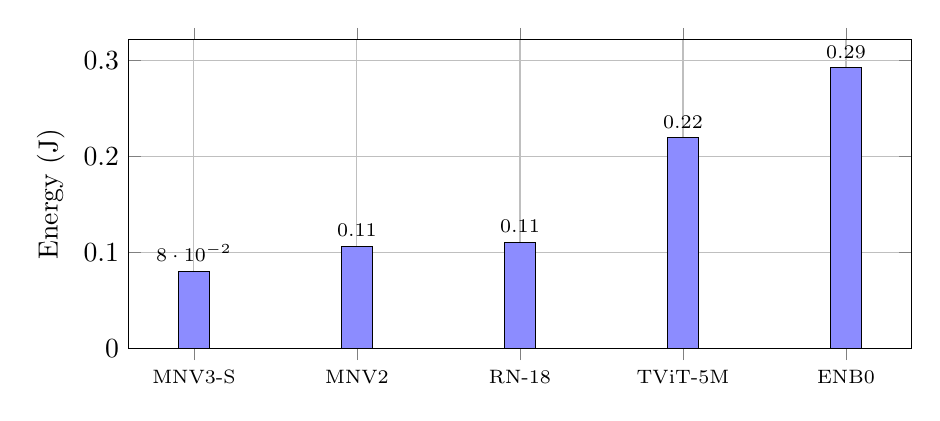
\begin{tikzpicture}
\begin{axis}[
    ybar,
    bar width=11pt,
    width=0.95\linewidth,
    height=5.5cm,
    ylabel={Energy (J)},
    symbolic x coords={MNV3-S,MNV2,RN-18,TViT-5M,ENB0},
    xtick=data,
    x tick label style={font=\scriptsize},
    ymin=0,
    nodes near coords,
    every node near coord/.append style={font=\scriptsize},
    grid=major,
]
\addplot[fill=blue!45] coordinates {
    (MNV3-S,0.080)
    (MNV2,0.106)
    (RN-18,0.110)
    (TViT-5M,0.219)
    (ENB0,0.292)
};
\end{axis}
\end{tikzpicture}
\caption{Measured energy per inference. MNV3-S = MobileNetV3-Small, MNV2 = MobileNetV2, RN-18 = ResNet-18, TViT-5M = Tiny-ViT-5M, ENB0 = EfficientNet-B0.}
\label{fig:measured-energy}
\end{figure}

\subsection{Direct Repeated Energy Audit}
Table~\ref{tab:energy-repeat} reports the direct repeated
\texttt{powermetrics} audit added for this submission. Each model has 10
measured 20-second windows, with raw logs and per-window rows stored in the
energy-audit artifact directory. Confidence intervals are Student-$t$ 95\%
intervals over the 10 measured windows. The audit was collected on the local
Apple M4 Pro environment in Table~\ref{tab:energy-environment}. Absolute
values differ from the paper-aligned mean table because the audit was
collected in a later hardware/software environment. We therefore use it as
local repeatability evidence, not as a replacement for the original source
table or as a basis for retroactively assigning confidence intervals to that
table.

High-power windows are visible in the repeated audit, with the largest
per-inference energy coming from MobileNetV3-Small repeat 6. We retain these
windows in the submitted data and summary rather than filtering them, because
the purpose of the audit is to expose measurement variability and make the raw
evidence chain inspectable.

\begin{table}[ht]
\centering
\caption{Direct repeated \texttt{powermetrics} audit on the local Apple M4 Pro MacBook Pro.}
\label{tab:energy-repeat}
\small
\resizebox{\linewidth}{!}{%
\begin{tabular}{l
r
S[table-format=4.1]
S[table-format=1.4]
S[table-format=1.4]
c
S[table-format=3.2]
S[table-format=1.3]}
\toprule
Model & {Windows} & {Inf./window} & {Mean $E$ (J)} & {$\sigma_E$ (J)} & {95\% CI for $E$ (J)} & {Latency (ms)} & {Power (W)} \\
\midrule
MobileNetV3-Small & 10 & 2066.7 & 0.0614 & 0.0259 & [0.0429, 0.0800] & 9.70 & 6.250 \\
MobileNetV2 & 10 & 1915.5 & 0.0661 & 0.0188 & [0.0526, 0.0795] & 10.45 & 6.288 \\
ResNet-18 & 10 & 1936.8 & 0.0735 & 0.0080 & [0.0678, 0.0793] & 10.34 & 7.102 \\
Tiny-ViT-5M & 10 & 800.7 & 0.1762 & 0.0286 & [0.1558, 0.1967] & 25.00 & 7.042 \\
EfficientNet-B0 & 10 & 593.0 & 0.2057 & 0.0294 & [0.1847, 0.2267] & 33.76 & 6.088 \\
\bottomrule
\end{tabular}
}
\end{table}

As a robustness check on the qualitative predictor result, the M4 Pro audit
means preserve the same pattern: latency explains most between-model energy
variation ($R^2 = 0.980$), while FLOPs remains uninformative
($R^2 = 0.001$). This check is reported separately because it reflects the
later M4 Pro environment rather than the original paper-aligned source run.

\subsection{Latency Tracks Energy; FLOPs Does Not}
\label{sec:predictors}
We fit two univariate linear models to the paper-aligned mean table, predicting
energy from FLOPs and from latency respectively. Results are summarized in
Table~\ref{tab:predictors}. In this five-model benchmark, latency explains
almost all observed variance in measured energy ($R^2 = 0.99999$), while FLOPs
explains only $R^2 = 0.00008$.

\begin{table}[ht]
\centering
\caption{Univariate linear predictors of measured energy ($n = 5$).}
\label{tab:predictors}
\begin{tabular}{l c c}
\toprule
Predictor & $R^2$ & Pearson $r$ \\
\midrule
Latency (ms) & 0.99999 & 0.99999 \\
FLOPs (G) & 0.00008 & -0.009 \\
Parameters (M) & 0.0547 & 0.234 \\
\bottomrule
\end{tabular}
\end{table}

To check whether the conclusion depends on a single model, we repeated the
linear fit after leaving out each architecture once. Latency remained stable
across these leave-one-out fits, with $R^2$ ranging from 0.99997 to 0.999999.
FLOPs remained weak, with leave-one-out $R^2$ ranging from 0.028 to 0.207.
Parameter count was also unstable, with leave-one-out $R^2$ ranging from
0.0003 to 0.494. As a rank-based check, Spearman correlation was 1.00 for
latency, 0.60 for FLOPs, and 0.70 for parameter count. These sensitivity
checks support the qualitative conclusion that latency is the stronger
predictor within this five-model benchmark.

The contrast is sharpest for two pairs:
\begin{itemize}
\item \textbf{ResNet-18 vs.\ EfficientNet-B0:} ResNet-18 has 4.7$\times$ the
FLOPs and 2.2$\times$ the parameters of EfficientNet-B0, yet consumes
0.38$\times$ the energy. A FLOP-based predictor would rank these in the
opposite order from measurement.
\item \textbf{MobileNetV2 vs.\ ResNet-18:} ResNet-18 has 6$\times$ the FLOPs
of MobileNetV2 but only 1.04$\times$ the energy. FLOPs overstates the gap by a
factor of nearly six.
\end{itemize}

\begin{figure}[ht]
\centering
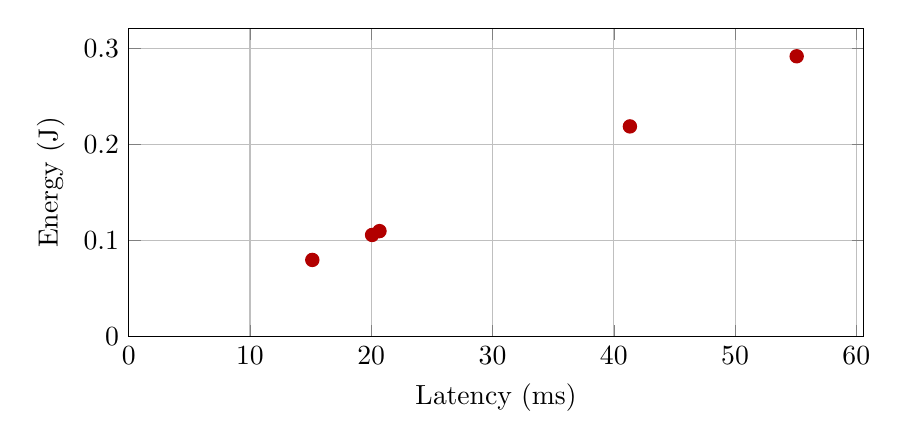
\begin{tikzpicture}
\begin{axis}[
    width=0.90\linewidth,
    height=5.5cm,
    xlabel={Latency (ms)},
    ylabel={Energy (J)},
    ymin=0,
    xmin=0,
    grid=major,
]
\addplot[
    only marks,
    mark=*,
    mark size=2.4pt,
    color=red!70!black
] coordinates {
    (15.14,0.080)
    (20.07,0.106)
    (20.68,0.110)
    (41.33,0.219)
    (55.08,0.292)
};
\end{axis}
\end{tikzpicture}
\caption{Measured energy versus latency for the paper-aligned five-model mean table. Linear fit gives $R^2 = 0.99999$.}
\label{fig:energy-vs-latency}
\end{figure}

\subsection{Architectural Interpretation}
The latency-FLOPs decoupling is consistent with three architecture-specific
effects on a CPU memory hierarchy.

\textbf{Depthwise convolutions are FLOP-efficient but memory-bound.} The
MobileNet family relies on depthwise separable convolutions, which reduce
arithmetic intensity (FLOPs per byte of memory traffic). On a CPU without
specialized depthwise kernels, the runtime spends a higher fraction of its
time in memory-bound stalls relative to compute, so wall-clock latency drops
less than FLOPs would suggest. This explains why MobileNetV2 (0.30 G FLOPs)
runs at similar latency to MobileNetV3-Small (0.22 G FLOPs) despite the FLOP
gap.

\textbf{Compound scaling creates cache pressure.} EfficientNet-B0 uses
compound scaling that grows depth, width, and input resolution together. While
this preserves a favorable accuracy-FLOPs tradeoff, the wider activation
tensors and deeper computational graph push working sets out of L2 cache on
the CPU, generating last-level cache misses and main-memory traffic that do
not appear in the FLOP count. In the paper-aligned mean table,
EfficientNet-B0's 0.39 G FLOPs corresponds to
55 ms of latency, while ResNet-18's 1.82 G FLOPs corresponds to only 21 ms.

\textbf{Transformer attention is FLOP-light but cache-unfriendly.} Tiny-ViT-5M
has fewer FLOPs than ResNet-18 (1.30 G vs.\ 1.82 G) but, in the same table,
nearly twice the
latency (41 ms vs.\ 21 ms). The attention operation requires multiple
matrix-multiply passes over the same input tokens with different projection
weights, with limited spatial locality compared to convolutions over feature
maps. On a CPU without fused attention kernels, this becomes the latency
bottleneck.

These interpretations are not novel as systems observations
\cite{eyeriss2017,hardwareaware2019}, but they have not been previously
reported for this specific set of architectures on Apple Silicon under a
unified runtime, and they explain why latency dominates FLOPs as an energy
proxy in this benchmark.

\subsection{Energy-Delay Product}
Table~\ref{tab:edp} reports EDP for the five architectures. EDP penalizes
both slow and energy-hungry models. Under EDP, MobileNetV3-Small has the
lowest EDP in the set, with an EDP 13.3$\times$ lower than
EfficientNet-B0. This metric is not accuracy-normalized; it measures
energy-latency cost per inference for the fixed input shape.

\begin{table}[ht]
\centering
\caption{Energy-Delay Product (EDP), lower is better.}
\label{tab:edp}
\begin{tabular}{l S[table-format=2.3] S[table-format=2.2]}
\toprule
Model & {EDP (J$\cdot$ms)} & {EDP relative to MNV3-S} \\
\midrule
MobileNetV3-Small & 1.211 & 1.00 \\
MobileNetV2 & 2.127 & 1.76 \\
ResNet-18 & 2.275 & 1.88 \\
Tiny-ViT-5M & 9.051 & 7.47 \\
EfficientNet-B0 & 16.083 & 13.28 \\
\bottomrule
\end{tabular}
\end{table}

\subsection{Supplemental Synthetic Fidelity}
\label{sec:fidelity}
The exploratory GAN was evaluated against the Apple-only grounded dataset.
Table~\ref{tab:fidelity} summarizes fidelity. Direct distributional tests are
applied only to the modeled quantities, energy and latency. Power is evaluated
as a derived quantity. Repeated-trial energy spread is evaluated as a
per-model summary after variance calibration. As discussed in the validation
scope subsection, this fidelity is measured against the grounded training
distribution, not against held-out measured trials.

\begin{table}[ht]
\centering
\caption{Supplemental GAN fidelity relative to the grounded Apple-only benchmark.}
\label{tab:fidelity}
\small
\begin{tabular}{l c c c c}
\toprule
Feature & W & KS & $p$ & Pass \\
\midrule
Energy & 0.0039 & 0.064 & 0.156 & Yes \\
Latency & 0.6934 & 0.067 & 0.120 & Yes \\
Derived power & 0.0457 & 0.047 & 0.498 & Yes \\
Energy spread & 0.0000 & N/A & N/A & Matched \\
\bottomrule
\end{tabular}

\vspace{0.3em}
\footnotesize
W = Wasserstein distance, KS = Kolmogorov--Smirnov statistic, $p$ = KS $p$-value.
Pass criterion is $p > 0.05$.
\end{table}

\subsection{Measured versus Synthetic Means}
Table~\ref{tab:alignment} compares measured means against the synthetic means.
Energy errors range from 1.0\% to 2.3\%; latency errors range from 1.4\% to
3.9\%.

\begin{table}[ht]
\centering
\caption{Measured versus paper-aligned synthetic mean metrics.}
\label{tab:alignment}
\resizebox{\linewidth}{!}{%
\begin{tabular}{l
S[table-format=1.3]
S[table-format=1.5]
S[table-format=2.2]
S[table-format=2.2]
S[table-format=2.2]
S[table-format=2.2]}
\toprule
Model &
{Measured $E$ (J)} &
{Synthetic $E$ (J)} &
{$E$ err (\%)} &
{Measured $L$ (ms)} &
{Synthetic $L$ (ms)} &
{$L$ err (\%)} \\
\midrule
MobileNetV3-Small & 0.080 & 0.08150 & 1.87 & 15.14 & 15.49 & 2.33 \\
MobileNetV2 & 0.106 & 0.10708 & 1.02 & 20.07 & 20.85 & 3.90 \\
ResNet-18 & 0.110 & 0.11169 & 1.54 & 20.68 & 20.97 & 1.39 \\
Tiny-ViT-5M & 0.219 & 0.22401 & 2.29 & 41.33 & 42.51 & 2.85 \\
EfficientNet-B0 & 0.292 & 0.29831 & 2.16 & 55.08 & 55.92 & 1.53 \\
\bottomrule
\end{tabular}
}
\end{table}

\subsection{Supplemental Power and Synthetic Trial Spread}
Table~\ref{tab:supplemental} reports derived average power and synthetic
energy spread. Derived power values come directly from measured energy and
latency. Synthetic spread values come from the calibrated GAN and are
interpreted as support estimates for repeated trials, not as measured
trial-level energy standard deviations.

\begin{table}[ht]
\centering
\caption{Supplemental power and synthetic trial-spread estimates. Model abbreviations match Fig.~\ref{fig:measured-energy}.}
\label{tab:supplemental}
\small
\resizebox{0.94\linewidth}{!}{%
\begin{tabular}{l
S[table-format=1.4]
S[table-format=1.4]
S[table-format=-2.2]
S[table-format=1.4]}
\toprule
Model &
{$P$ (W)} &
{Syn $P$ (W)} &
{Err (\%)} &
{Syn $\sigma_E$ (J)} \\
\midrule
MNV3-S & 5.2840 & 5.2976 & 0.26 & 0.0045 \\
MNV2 & 5.2815 & 5.1677 & -2.15 & 0.0081 \\
RN-18 & 5.3191 & 5.3558 & 0.69 & 0.0073 \\
TViT-5M & 5.2988 & 5.3054 & 0.12 & 0.0167 \\
ENB0 & 5.3014 & 5.3752 & 1.39 & 0.0201 \\
\bottomrule
\end{tabular}
}
\end{table}

\section{Discussion}
The empirical results show that, in this five-model Apple-Silicon CPU-only
PyTorch benchmark, latency is very strongly associated with energy
($R^2 = 0.99999$), while FLOPs explains almost none of the measured energy
variation ($R^2 = 0.00008$) in the paper-aligned mean table. The architectural
interpretation in Section~\ref{sec:predictors} explains why: depthwise
convolutions, compound scaling, and transformer attention each create memory
behavior on a general-purpose CPU that decouples FLOPs from wall-clock time.
Average power in that table is roughly constant across the five models
(5.28--5.32 W), so
the model that takes longer simply pays for more wall-clock energy at a
similar power level. This means EDP, which weights both factors, ranks the
models in the same order as energy alone but with a wider EDP spread
(13.3$\times$ best-to-worst).

The later M4 Pro repeated audit has different absolute power levels, but it
supports the same qualitative conclusion: latency remains the strong
between-model predictor and FLOPs remains weak.

The synthetic pipeline produced a tightly scoped repeated-trial model that
reproduces the measured energy ranking and tracks measured means within
1.0--2.3\% on energy and 1.4--3.9\% on latency. The strongest claim about
the synthetic dataset is that it preserves the model ranking and reproduces
mean energy and latency closely. We do not claim that the synthetic spread
estimates predict the variance of physical repeated trials, because the GAN
was trained and evaluated against a grounded distribution rather than
independently held-out measurements.

The methodological lesson from this GAN development step is narrower but
practical: when training data are sparse, a synthetic model should be tightly
scoped to the target study and trained on normalized residual structure rather
than raw heterogeneous values. We observed this directly: a multi-device
raw-scale configuration mode-collapsed, while the same architecture trained
on normalized within-combination residuals in a single-device scope reproduced
per-model structure faithfully.

\section{Limitations and Future Work}
\label{sec:limitations}
\textbf{Trial-level measurement.} The original paper-aligned benchmark
recorded means but did not preserve per-trial energy spreads, confidence
intervals, window counts, raw \texttt{powermetrics} logs, or the exact
original power-sampling command. This study adds a follow-up direct
energy audit with 10 measured windows per model, measured standard deviations,
confidence intervals, and raw logs. However, that audit was collected later on
a local Apple M4 Pro MacBook Pro, not recovered from the original source run, so
its intervals should be interpreted as local repeatability evidence rather
than retroactive uncertainty estimates for the original mean table. A future
revision should rerun the complete original benchmark with the same logging
policy.

\textbf{Single-device scope.} The paper is a single-device study. Replicating
the benchmark on additional devices, with the same input shape, runtime
constraints, and reporting format, would test whether the FLOPs--energy
mismatch generalizes beyond Apple Silicon and would also enable a true
multi-device synthetic model.

\textbf{Power sampling resolution.} The 1 Hz \texttt{powermetrics} sampling
interval is coarse relative to per-inference latency. We addressed this with
window-level energy attribution, but higher-resolution power traces would
support per-inference rather than per-window analysis.

\textbf{Accuracy normalization.} This study reports energy, latency, and EDP
per inference. It does not normalize by ImageNet top-1 accuracy or any other
task-performance metric, so the word ``efficient'' should be read as
energy-latency efficient under the fixed input and runtime, not as
accuracy-normalized model quality per joule.

\textbf{Synthetic validation.} GAN fidelity is evaluated against grounded
training data. Direct validation against an independent set of measured
repeated trials is required before synthetic spreads can be cited as
predictions rather than support estimates.

\textbf{Sample size.} With $n = 5$ models, the predictor $R^2$ values in
Table~\ref{tab:predictors} are estimated from a small sample. We include
leave-one-out and Spearman sensitivity checks, but the precise coefficients
should still be interpreted as exploratory until the benchmark is expanded to
more architectures.

\textbf{Hardware accelerator coverage.} The benchmark intentionally restricts
to CPU-only execution to control runtime variability. Apple Silicon's Neural
Engine and Metal Performance Shaders backends would likely produce different
energy rankings, which is itself a topic for future work.

\section{Conclusion}
This study finds that on Apple Silicon under CPU-only PyTorch inference,
per-inference energy/latency behavior cannot be reduced to FLOPs or parameter
count alone.
In this five-model benchmark, latency tracks energy at $R^2 = 0.99999$,
while FLOPs achieves only $R^2 = 0.00008$. Under Energy-Delay Product,
MobileNetV3-Small has 13.3$\times$ lower EDP than EfficientNet-B0, with the
rest of the architectures in between. A later M4 Pro repeated audit provides
local repeatability evidence and preserves the same qualitative
latency-over-FLOPs pattern. A residualized conditional WGAN-GP,
trained within a single-device
scope after an initial raw-scale multi-device configuration exhibited mode
collapse, reproduces the measured ranking and means within a few percent.
The methodological lesson is that synthetic models of hardware behavior
under sparse data must be tightly scoped and trained on normalized residual
structure rather than raw heterogeneous values.

\section{Reproducibility Appendix}
\label{sec:appendix}

\subsection{Released Artifacts and Commands}
The anonymized artifact bundle separates direct measurements, derived proxy columns,
and synthetic support data. The five-model energy means used in the main
figures and predictor analysis are stored in:
\begin{verbatim}
paper_apple_silicon_benchmark.csv
\end{verbatim}
The direct repeated energy audit can be reproduced with:
\begin{verbatim}
python3 scripts/measure_energy_powermetrics.py \
  --windows 10 --window-seconds 20 \
  --sample-interval-ms 1000 --warmups 10 \
  --cooldown-seconds 10 --threads 1
\end{verbatim}
This command writes:
\begin{verbatim}
measured_energy_powermetrics/
  measured_energy_trials.csv
  measured_energy_summary.csv
  measurement_environment_energy.json
  raw_powermetrics/
\end{verbatim}
The expanded direct latency sweep can be reproduced with:
\begin{verbatim}
.venv/bin/python scripts/benchmark_architectures.py \
  --trials 30 --warmup 10 --threads 1
\end{verbatim}
This command writes:
\begin{verbatim}
measured_architecture_benchmark.csv
measured_architecture_trials.csv
measurement_environment.json
paper_baseline_comparison.csv
\end{verbatim}
The raw per-trial rows for the expanded sweep live in the measured architecture
trials CSV. The follow-up energy audit
contains the matching raw power traces, one integrated energy row per
measurement window, the exact \texttt{powermetrics} command template, window
duration, inferences per window, warmup count, cooldown policy, and randomized
model order. The original source traces behind the Apple benchmark CSV remain
unavailable.

\subsection{GAN Architecture and Training}
The conditional WGAN-GP implementation uses one-hot device/model conditioning
concatenated to the latent input. The generator projects a 64-dimensional noise
vector plus the condition vector into a 256-unit hidden representation, applies
three residual blocks with layer normalization and LeakyReLU activations, and
maps the result through a 256-to-128-to-output head. The critic concatenates
the feature vector and condition vector, then applies four 256-unit
spectral-normalized linear blocks with LeakyReLU activations and dropout before
the scalar WGAN score. The gradient penalty coefficient is $\lambda = 10$.
Training uses Adam with learning rate $10^{-4}$ and betas $(0.0, 0.9)$, five
critic updates per generator update, batch size 64, and seed 42. The default
training script supports 2000 epochs; the paper-aligned runs used the same
source workflow and stored checkpoint/history artifacts locally during
development.

\subsection{Combo-Normalization Procedure}
For each (device, model) combination $c$, mean $\mu_c$ and standard deviation
$\sigma_c$ are computed for each continuous feature. Training samples are
transformed as $\tilde{x} = \mathrm{clip}((x - \mu_c)/\sigma_c, -3, 3)$.
Generated samples are inverse-transformed as $x = \mu_c + \sigma_c \cdot \tilde{x}$
using the combo identity sampled with the conditioning vector.

\subsection{Variance Calibration}
After generation, per-model variance for energy and latency is rescaled to
match the grounded Apple-only seed distribution variance. Means are unaffected
by this rescaling.

\subsection{Random Seeds and Software Environment}
The submitted GAN workflow fixes the GAN seed at 42 and specifies package
ranges in the submitted requirements file: PyTorch $\geq 2.0$, NumPy
$\geq 1.24$, pandas $\geq 2.0$, scikit-learn $\geq 1.3$, and SciPy
$\geq 1.11$. The expanded latency sweep logs exact runtime details in
\texttt{measurement\_environment.json}: Apple M4 Pro MacBook Pro Mac16,8,
24 GB RAM, macOS 26.2 build 25C56, Python 3.9.6, PyTorch 2.8.0, CPU float32
execution, CUDA unavailable, MPS unavailable, one PyTorch CPU thread, 12
inter-op threads, input shape $1 \times 3 \times 224 \times 224$, 10 warmups,
and 30 measured trials. The original five-model energy source does not archive
the exact torchvision version or raw power-sampling command. The follow-up
direct energy audit logs exact runtime details in the energy audit environment
JSON: Apple M4 Pro MacBook Pro Mac16,8, 24 GB RAM, macOS 26.2 build
25C56, Python 3.9.6, PyTorch 2.8.0, torchvision 0.23.0, timm 1.0.24, CPU
float32 execution, one PyTorch CPU thread, one inter-op thread, input shape
$1 \times 3 \times 224 \times 224$, 10 repeated windows per model, 20 seconds
per window, 1 Hz \texttt{powermetrics} sampling, 10 warmups, 10 seconds
cooldown, and randomized order with seed 20260430.

\subsection{Sensitivity Checks}
For the predictor analysis in Table~\ref{tab:predictors}, Pearson $r$ and
$R^2$ are computed from the five measured model means. Leave-one-out
sensitivity is computed by omitting one architecture, refitting the univariate
linear relationship on the remaining four points, and recording the resulting
$R^2$. Spearman correlations are computed from model rankings. These checks
are reported to prevent overinterpreting the exact coefficients from a
five-model benchmark.


\subsubsection{Declaration on Generative AI Assistance.}
\begin{sloppypar}
Generative AI tools were used only for grammar proofreading and LaTeX
formatting checks. They were not used to design the experiments, generate
measurements, perform the analysis, or determine the conclusions. The human
authors reviewed the manuscript and take full responsibility for the accuracy,
originality, and integrity of the work.
\end{sloppypar}

\begin{thebibliography}{20}

\bibitem{horowitz2014}
M.~Horowitz, ``Computing's energy problem (and what we can do about it),''
\emph{IEEE Micro}, vol.~34, no.~5, pp.~10--14, 2014.

\bibitem{mobilenet2017}
A.~G. Howard et al., ``MobileNets: Efficient convolutional neural networks for
mobile vision applications,'' \emph{arXiv preprint arXiv:1704.04861}, 2017.

\bibitem{mobilenetv22018}
M.~Sandler, A.~Howard, M.~Zhu, A.~Zhmoginov, and L.-C. Chen,
``MobileNetV2: Inverted residuals and linear bottlenecks,'' in
\emph{Proc. IEEE Conf. Computer Vision and Pattern Recognition}, 2018.

\bibitem{mobilenetv32019}
A.~Howard, M.~Sandler, G.~Chu, et al., ``Searching for MobileNetV3,'' in
\emph{Proc. IEEE International Conf. Computer Vision}, 2019.

\bibitem{efficientnet2019}
M.~Tan and Q.~Le, ``EfficientNet: Rethinking model scaling for convolutional
neural networks,'' in \emph{Proc. International Conf. Machine Learning}, 2019.

\bibitem{squeezenet2016}
F.~N. Iandola, S.~Han, M.~W. Moskewicz, K.~Ashraf, W.~J. Dally, and
K.~Keutzer, ``SqueezeNet: AlexNet-level accuracy with 50x fewer parameters and
<0.5MB model size,'' \emph{arXiv preprint arXiv:1602.07360}, 2016.

\bibitem{shufflenet2018}
X.~Zhang, X.~Zhou, M.~Lin, and J.~Sun, ``ShuffleNet: An extremely efficient
convolutional neural network for mobile devices,'' in \emph{Proc. IEEE Conf.
Computer Vision and Pattern Recognition}, 2018.

\bibitem{mnasnet2019}
M.~Tan, B.~Chen, R.~Pang, V.~Vasudevan, M.~Sandler, A.~Howard, and Q.~V. Le,
``MnasNet: Platform-aware neural architecture search for mobile,'' in
\emph{Proc. IEEE Conf. Computer Vision and Pattern Recognition}, 2019.

\bibitem{proxylessnas2019}
H.~Cai, L.~Zhu, and S.~Han, ``ProxylessNAS: Direct neural architecture search
on target task and hardware,'' in \emph{Proc. International Conf. Learning
Representations}, 2019.

\bibitem{fbnet2019}
B.~Wu, X.~Dai, P.~Zhang, Y.~Wang, F.~Sun, Y.~Wu, Y.~Tian, P.~Vajda, Y.~Jia,
and K.~Keutzer, ``FBNet: Hardware-aware efficient ConvNet design via
differentiable neural architecture search,'' in \emph{Proc. IEEE Conf.
Computer Vision and Pattern Recognition}, 2019.

\bibitem{onceforall2020}
H.~Cai, C.~Gan, T.~Wang, Z.~Zhang, and S.~Han, ``Once-for-All: Train one
network and specialize it for efficient deployment,'' in \emph{Proc.
International Conf. Learning Representations}, 2020.

\bibitem{mittal2019}
S.~Mittal, ``A survey of techniques for improving energy efficiency of deep
learning,'' \emph{ACM Computing Surveys}, vol.~51, no.~2, 2019.

\bibitem{hardwareaware2019}
Y.~He et al., ``Understanding FLOPs is not enough: A study of hardware-aware
neural networks,'' \emph{arXiv preprint arXiv:1912.01090}, 2019.

\bibitem{eyeriss2017}
Y.-H. Chen et al., ``Eyeriss: An energy-efficient reconfigurable accelerator
for deep convolutional neural networks,'' \emph{IEEE J. Solid-State Circuits},
2017.

\bibitem{greenai2020}
R.~Schwartz, J.~Dodge, N.~A. Smith, and O.~Etzioni, ``Green AI,''
\emph{Communications of the ACM}, vol.~63, no.~12, pp.~54--63, 2020.

\bibitem{strubell2019}
E.~Strubell, A.~Ganesh, and A.~McCallum, ``Energy and policy considerations
for deep learning in NLP,'' in \emph{Proc. Annual Meeting of the Association
for Computational Linguistics}, 2019.

\bibitem{patterson2021}
D.~Patterson, J.~Gonzalez, Q.~Le, C.~Liang, L.-M. Munguia, D.~Rothchild,
D.~So, M.~Texier, and J.~Dean, ``Carbon emissions and large neural network
training,'' \emph{arXiv preprint arXiv:2104.10350}, 2021.

\bibitem{mlperf2020}
V.~J. Reddi et al., ``MLPerf Inference Benchmark,'' in \emph{Proc. ACM/IEEE
International Symposium on Computer Architecture}, 2020.

\bibitem{wgangp2017}
I.~Gulrajani, F.~Ahmed, M.~Arjovsky, V.~Dumoulin, and A.~Courville,
``Improved training of Wasserstein GANs,'' in \emph{Advances in Neural
Information Processing Systems}, 2017.

\bibitem{ctgan2019}
L.~Xu, M.~Skoularidou, A.~Cuesta-Infante, and K.~Veeramachaneni, ``Modeling
tabular data using conditional GAN,'' in \emph{Advances in Neural Information
Processing Systems Workshop}, 2019.

\end{thebibliography}

\end{document}
